
\chapter{Measuring sound}
\section{The measurement microphone}
	The measuring device is called a \textbf{sonometer} and is generally composed of a microphone, an amplifier, a conditioner and a display. We denote "type x" to specify the accuracy of the device, the more accurate being type 0 and then 1, 2, ... 
	\begin{wrapfigure}[10]{l}{3.5cm}
	\vspace{-5mm}
	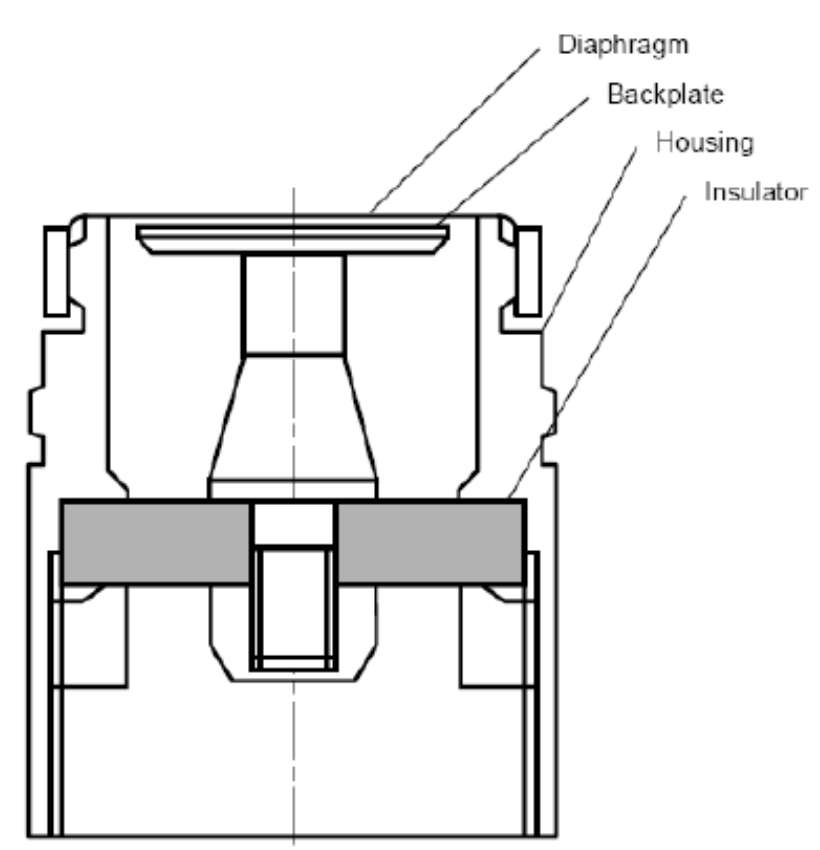
\includegraphics[scale=0.25]{acoustics/ch3/1}
	\captionof{figure}{}
	\label{fig:3.1}
	\end{wrapfigure}
	\autoref{fig:3.1} represents the principle of a condenser microphone. It is composed of two charged plates, one being the thin membrane in contact with the incoming sound waves, the second is the backplate which is the base plate. An electrical charge is created by means of a voltage supply. The sound makes the distance between the plates change and thus implies a capacity change and a voltage change according to:
	
	\begin{equation}
	Q = CV, C = \epsilon \frac{A}{d} \qquad \Rightarrow \Delta V = \frac{Q}{\epsilon A} \Delta d.
	\end{equation}
	
	\ \\
	
	\begin{wrapfigure}[10]{r}{6cm}
	\vspace{-5mm}
	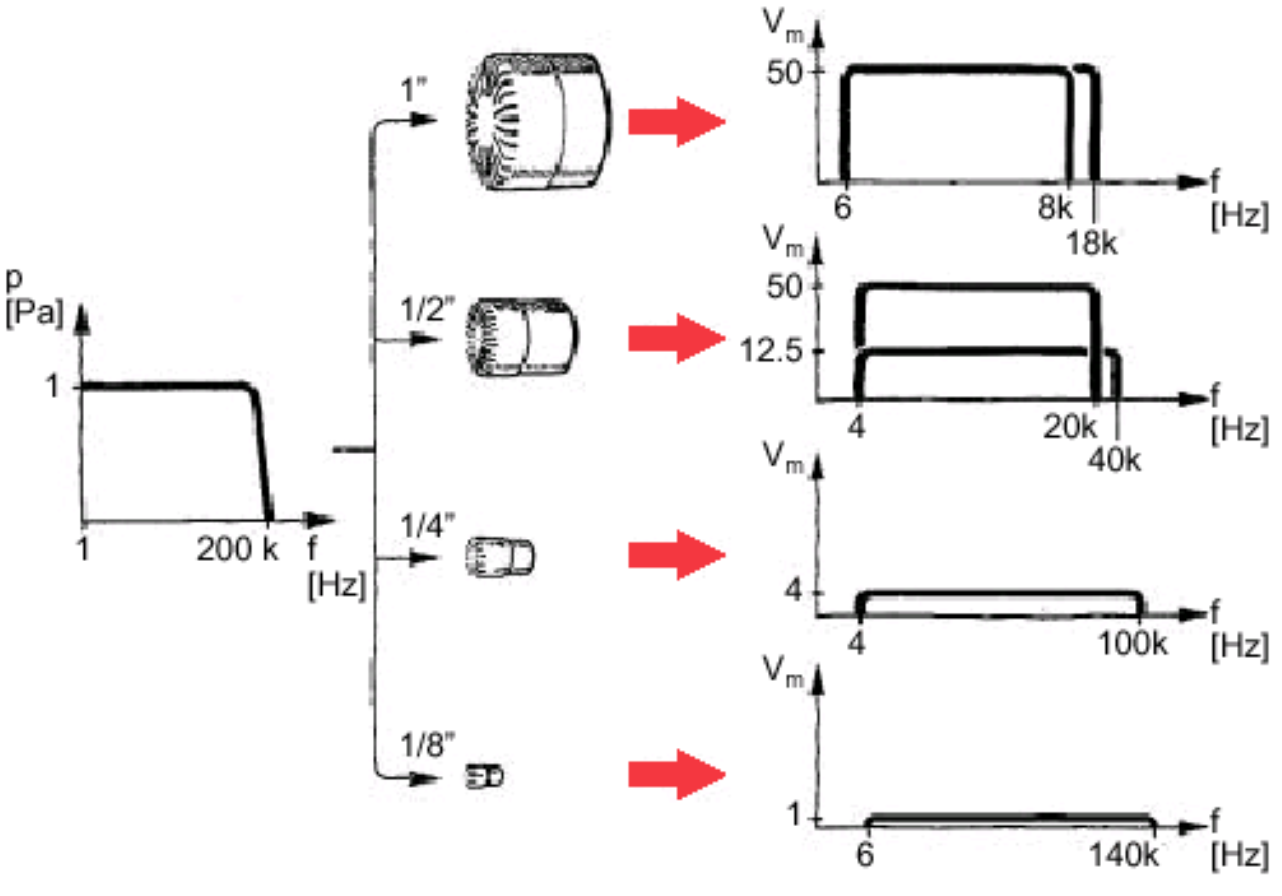
\includegraphics[scale=0.25]{acoustics/ch3/2}
	\captionof{figure}{}
	\label{fig:3.2}
	\end{wrapfigure}
	The size of the microphone is important. The smaller the microphone, the higher is the range of frequency. Indeed, if we take the formula $f \lambda = c$, we've seen that the wave length is smaller when the frequency is higher, for example if we have 1000 Hz $\rightarrow \lambda =$ 3 cm. We need to have a wave homogeneity on the membrane. So for the example we gave, we need to have a membrane smaller than 1.5 cm. On the other hand, larger microphones have bigger sensibility and allow to hear less loud sounds. 
	
	\begin{center}
	\begin{minipage}{0.4\textwidth}
	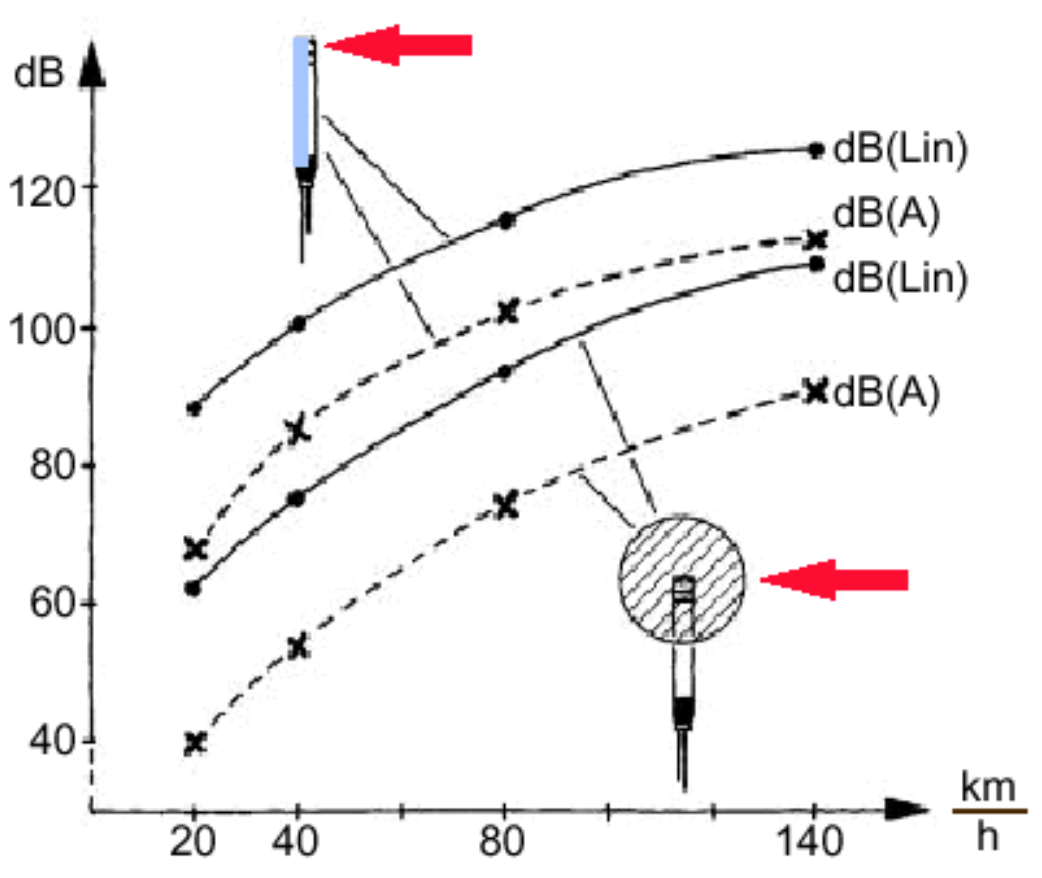
\includegraphics[scale=0.25]{acoustics/ch3/3}
	\captionof{figure}{}
	\label{fig:3.3}
	\end{minipage}
	\begin{minipage}{0.4\textwidth}
	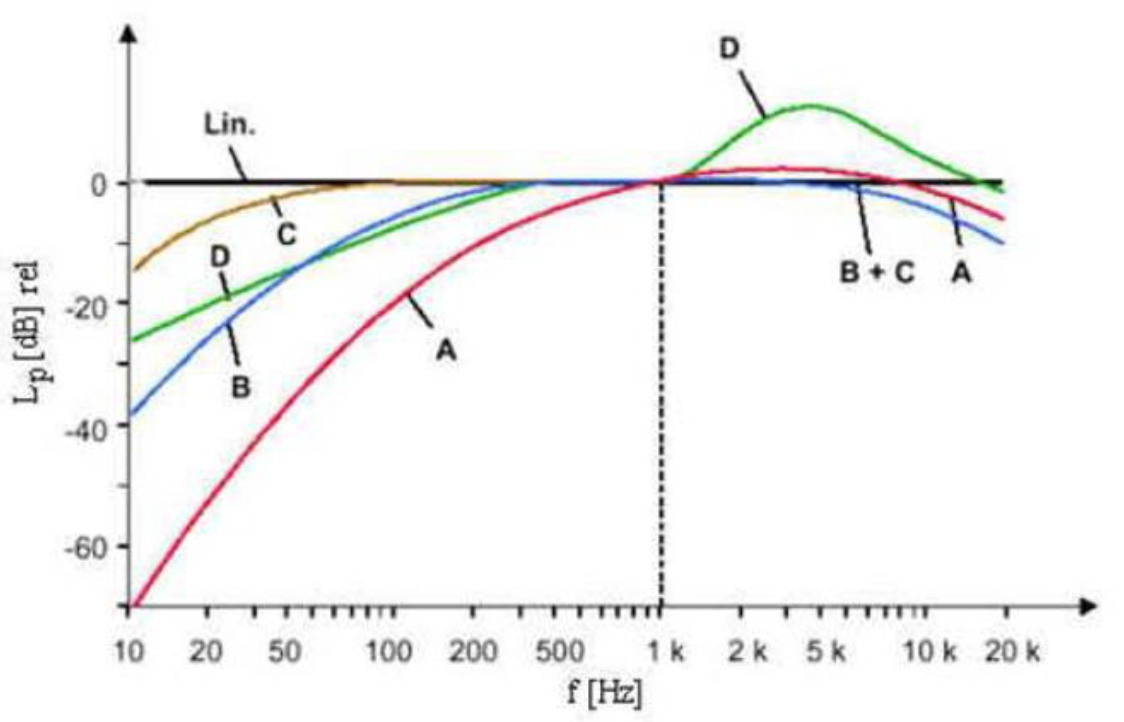
\includegraphics[scale=0.35]{acoustics/ch3/4}
	\captionof{figure}{}
	\label{fig:3.4}
	\end{minipage}
	\end{center}

	The wind is a polluting noise that has great effects. We can see that above 40 km/h the influence is enormous. To avoid the parasites, we use a ball windscreen and an A-weighting to soften the signal. This is shown on \autoref{fig:3.3}. On \autoref{fig:3.4} are shown the different weightings used in practice, the dbA is accomplished by adjusting the sound level in every band to the frequency sensitivity of the human ear for soft sound (40 dB). According to the practical case, one of them will be used. For example if we organize a party, the presence of a lot of low frequencies forces the use of dB(A).\\
	
	We can have devices that gives the sound level by frequency band. In this case the device has a calibration chart and need to be calibrated sometimes. \\
	
	Another qualification unit is the \textbf{sound pressure level}, which is the exposure level. This is comparable to the RMS value but we integrate this in a certain range of time without dividing: 
	
	\begin{equation}
	SEL = 10 \log \left( \int _0^T 10^{L/10}\, dt \right)
	\end{equation}
	
	we use in this case a \textbf{dose meter}. 
	
\section{Sound intensity measurement}	
	We have seen that $I_x = pv_x$, where p can be measured by means of a microphone but the air particles velocity is more difficult. We can do this:
	
	\begin{equation}
	F_x = ma \qquad \Rightarrow \rho \frac{\D v_x}{\D t} = - \frac{\D p}{\D x} \qquad \Rightarrow v_x = -\frac{1}{\rho} \int \frac{\D p}{\D x}
	\end{equation}
	
	In fact to compute the intensity we use the discretized function: 
	
	\begin{equation}
	I_x = \overline{pv_x} = -\frac{1}{2\rho\Delta r}\overline{(p_A + p_B)\int  (p_A - p_B)\, dt}
	\end{equation}
	where $p_A,p_B$ are the pressure at to neighboring positions. The intensity meter consists so in two microphones separated by a certain distance. This device can be used to determine the direction of the source as the intensity is a vectorial quantity.  Let's specify that the frequency range is rather limited, its upper limit is given by $f_U = \frac{c}{4D}$. 
	
\section{Sound power measurement}
\subsection{Using microphones}
	\begin{wrapfigure}[8]{l}{5cm}
	\vspace{-5mm}
	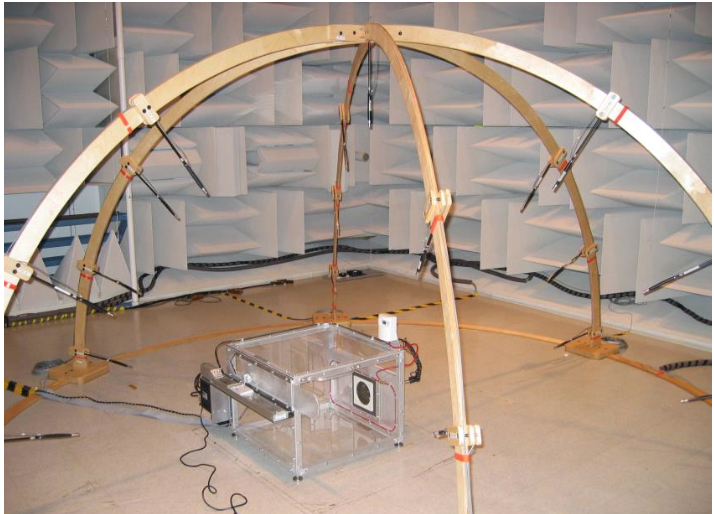
\includegraphics[scale=0.35]{acoustics/ch3/5}
	\captionof{figure}{}
	\label{fig:3.5}
	\end{wrapfigure}
	A first method to determine the power is the use of microphone in a delimited volume, but this method can only be applied in no wall conditions, no reflection (semi-anechoic room)! The surrounding surface can be a parallellepipedum, an hemisphere or a sphere, so we can use the formula $W : IS$. If the micrphones are far from the emitting body (plane wave assumption), we can calculate thee power using: 
	
	\begin{equation}
	L_w=  \bar{L}_p + 10 \log \frac{S}{S_0} - K_1 - K_2 \qquad anf \bar{L}_p = 20 \l \frac{1}{N}\sum _{i = 1}^N 10^{0.1 L_{p_i}}
	\end{equation}

	If I come near the machine, the wave are not plane waves anymore.

\subsection{Comparison method}
	In this method, we are not limited about the volume anymore, the microphones have to be placed far enough too. We are using a known source which diffuses a known power $L'_W$. We then perform a test in the acoustic hard room and compute the spacial averages $L_{pm}$ from the $L_{p_i}$ of the unknown source. Then we do the same for the known source and we can compute the unknown power as:
	
	\begin{equation}
	L_W = L'_W + (L_{pm} - L'_{pm}).
	\end{equation}
	
\subsection{Using sound intensity}
	In this method we directly measure the intensity using an intensity meter and not anymore the pressure. We have to define a surrounding surface that we discretize. Then we get the intensity on these points and compute the discrete powers $W_i = I_{ni}S_i$ that we use to get the average power level:
	
	\begin{equation}
	L_{W} = 10 \log \sum _{i=1}^N \frac{W_i}{W_0}.
	\end{equation}
	
	The advantages of this method are: elimination of background noise, in situation measurements possible, nearfield measurements and the arbitrary surface. The disadvantages are: limited frequency range, directivity and the cost of the device. 
	
\section{Question (written exam)}
	\begin{itemize}
	\item[•] Explain the working principle of the human hearing system.
 	\item[•] Discuss the working principle of a sonometer and an intensity meter.
	\item[•] Explain how one can measure sound power in practice.
	\end{itemize}